%
% fig-strahlungsspektren.tex
%
% (c) 2025 Prof Dr Andreas Müller
%
\begin{figure}
	\centering
	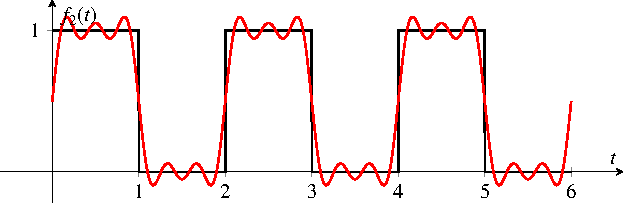
\includegraphics{papers/fourier/images/fourier_Rechteck.pdf}
	\caption{Fourierapproximation einer Rechteckfunktion}
	\label{fourier:fig:fourierrechteck}
\end{figure}